% This is a basic Math Paper

\documentclass[11pt]{article}

% Preamble

\usepackage[margin=1in]{geometry}
\usepackage{amsfonts, amsmath, amssymb}
\usepackage{fancyhdr, float, graphicx}
\usepackage[utf8]{inputenc} % Required for inputting international characters
\usepackage[T1]{fontenc} % Output font encoding for international characters
\usepackage{fouriernc} % Use the New Century Schoolbook font
\usepackage[nottoc, notlot, notlof]{tocbibind}
\usepackage{url}
\usepackage{placeins}
\usepackage{multirow}
% Header and Footer
\pagestyle{fancy}
\fancyhead{}
\fancyfoot{}
\fancyhead[L]{\textit{\Large{Experiment 3. Law of Malus}}}
%\fancyhead[R]{\textit{something}}
\fancyfoot[C]{\thepage}
\renewcommand{\footrulewidth}{1pt}



% Other Doc Editing
% \parindent 0ex
%\renewcommand{\baselinestretch}{1.5}

\begin{document}
	
	\begin{titlepage} 
		\centering 
		
		%---------------------------NAMES-------------------------------
		
		\huge\textsc{
			MIT World Peace University
		}\\
	
		\vspace{0.75\baselineskip} % space after Uni Name
		
		\LARGE{
			Physics\\
			First Year B. Tech, Trimester 3\\
			Academic Year 2021-22
		}
		
		\vfill % space after Sub Name
		
		%--------------------------TITLE-------------------------------
		
		\rule{\textwidth}{1.6pt}\vspace*{-\baselineskip}\vspace*{2pt}
		\rule{\textwidth}{0.6pt}
		\vspace{0.75\baselineskip} % Whitespace above the title
		
		
		
		\huge{\textsc{
				Law of Malus
			}} \\
		
		
		
		\vspace{0.5\baselineskip} % Whitespace below the title
		\rule{\textwidth}{0.6pt}\vspace*{-\baselineskip}\vspace*{2.8pt}
		\rule{\textwidth}{1.6pt}
		
		\vspace{1\baselineskip} % Whitespace after the title block

		%--------------------------SUBTITLE --------------------------	
			
		\LARGE\textsc{
			Experiment No. 3
		} % Subtitle or further description
		\vfill
		
		%--------------------------AUTHOR-------------------------------
		
		Prepared By
		\vspace{0.5\baselineskip} % Whitespace before the editors
		
		\Large{
			109054. Krishnaraj Thadesar
			
			Division 9 Batch I3
		}
		
		
		\vspace{0.5\baselineskip} % Whitespace below the editor list
		\today

	\end{titlepage}

	\begin{center}
	{\Large Pledge}\\
	\vspace{0.5cm}
	I solemnly affirm that I am presenting this journal based on my own experimental work. I have neither copied the observations, calculations, graphs and results from others nor given it to others for copying.\\
		\end{center}
	
	\vspace{0.5cm}
	
    \begin{flushright}
	{\large Signature of the student}\\
	\vspace{1cm}
	 \end{flushright}
	
	
	
	\begin{center}
		{\LARGE Experiment 2: Diffraction Grating}\\
	\end{center}

	\section{Aim}
	\noindent
To verify law of Malus
	
	\section{Apparatus}


		\begin{enumerate}
			\item Monochromatic source of light
			\item Two polarizers with angular scale from 0-360o
			\item Luxmeter
			\item Metallic tube for mounting polarizer and analyzer
		\end{enumerate}


	\section{Significance of the Experiment}
\textit{Law of Malus, which relates the intensities transmitted by a
polarizer and analyzer, is the basis of several applications such as polarizing sunglasses, visors
of the automobiles, seven segment LCDs, polarimeters, optical activity, blue sky, red sunset,
Faraday effect, Kerr effect, photoeleasticity etc. Law of Malus is also used in analysis of
polarized light}
	
	
	\section{Theory}

 An unpolarized light consists of the vibrations which are isotropically distributed in all $360^{\circ}$ directions transverse to direction of propagation. Since vibrations exist in all the directions, their net $\mathrm{X}$ and $\mathrm{Y}$ components are equal i.e. $50 \%$. If such light is passed through a polarizer, the components parallel to optic axis are transmitted and components perpendicular to optic axis are eliminated. Thus when the light is polarized once, its intensity decreases by $50 \%$. Consider a system of two polarizers having an angle $\theta$ between their optic axes. Let the amplitude and intensity of the light incident on the first polarizer be $E_{o}$ and $I_{o}$ respectively. When the light passes through first polarizer, its amplitude and intensity reduces. Let these reduced amplitude and intensity be $E_{l}$ and $I_{l}$ respectively. (We have $I_{1} \cong \frac{I_{o}}{2}$ ). As the angle between the optic axes of the polarizers is $\theta$, the light polarized by the first polarizer $\left(E_{l}\right)$ is incident on the second polarizer at $\theta$ itself (refer Fig 3.1). Second polarizer transmits the cosine component of $E_{1}$ as it is along its optic axis. If the $E_{2}$ and $I_{2}$ are the amplitude and intensity of the light transmitted by the second polarizer, then we have
$$
E_{2}=E_{1} \cos \theta \Rightarrow I_{2}=I_{1} \cos ^{2} \theta
$$
Eqn (3.1) signifies that $I_{2}$ is the function of $\theta$ and $I_{1}$ is the maximum value of $I_{2}$. Thus, by choosing appropriate notations,

$$ I_\theta = I_m cos^2\theta$$

Eqn (3.1) and (3.2) represent law of Malus. The law states that the intensity transmitted by a pair
of polarizers is a cosine square function of the angle between their optic axes.

	\begin{figure}[H]
		\centering
		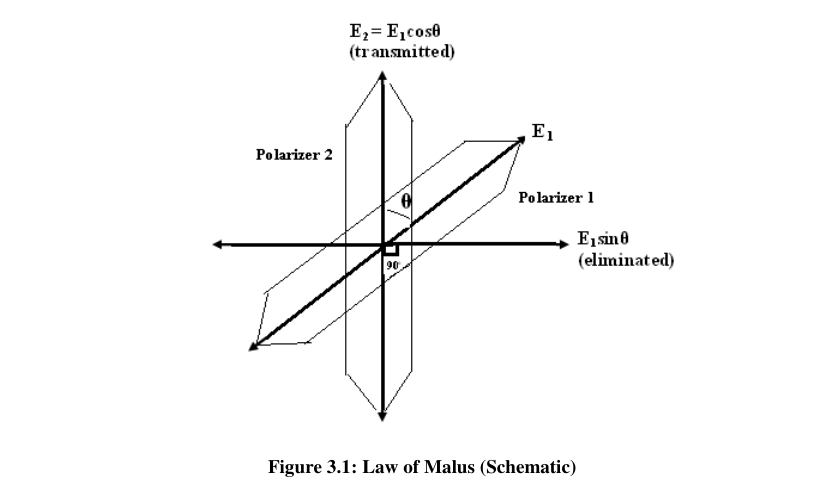
\includegraphics[scale=0.8]{theory.png}
		\label{it}
	\end{figure}
	
	\section{Procedure}
	
	\begin{enumerate}
	
	
	
	
	\item Remove slit as well as lens of a collimator (of the spectrometer) and mount polarizers at both the ends.
	\item The polarizer towards the light source is called polarizer and that towards the observer is called analyzer.
	\item Level the collimator tube using spirit level.
	\item Perform the experiment in dark room so that no other light except that from sodium will enter the detector (Luxmeter)
	\item Make the luxmeter $\mathrm{ON}$ and set it at appropriate range (0-200 Lux)
	\item Rotate the analyzer through $360^{\circ}$ while looking through it. The intensity will maximize three times at $\theta$ equal to $0^{\circ}, 180^{\circ}$ and $360^{\circ}$, while intensity will be extinguished at $\theta$ equal to $90^{\circ}$ and $270^{\circ}$.
	
	\item Adjust the analyzer so that it transmits maximum intensity. This corresponds to $\theta=0^{\circ}$ condition. Confirm this position by using a Luxmeter. Hold the sensor of the Luxmeter on the analyzer and move the analyzer slightly back and forth and detect the exact maximum intensity position. Note the corresponding angular position of the analyzer. Let this be $\theta^{\prime}$. As this is maximum intensity condition, it corresponds to $\theta=0^{\circ}$. $\theta^{\prime}$ is the angular position of the analyzer and $\theta$ is the angle between the optic axes of polarizer and analyzer. $\theta$ 'and $\theta$ need not be same. Also record the maximum intensity shown by the luxmater. This is $I_{m}$
	30
	
	\item Now rotate the analyzer by $30^{\circ}$ each time and record both $\theta^{\prime \prime}$ and $\theta$. Also record the corresponding intensities using the Luxmeter. These intensities are denoted by $I_{\theta}$ Continue the observations till $\theta$ reaches $360^{\circ}$. Record all your readings in the observation table 3.1.
	\item Calculate $\frac{I_{\theta}}{I_{m}}$ and $\cos ^{2} \theta$ for each $\theta$
	\item Plot the graph of $\frac{I_{\theta}}{I_{m}} \mathrm{Vs} \theta$ for all 13 values of $\theta$. It will show cosine square nature.
	\item Also plot the graph of $\frac{I_{\theta}}{I_{m}} \operatorname{Vs} \cos ^{2} \theta$ only for first four values. It will be a straight line
	\item Both these graphs signify law of Malus
	
	
	

	\end{enumerate}
\clearpage

	\section{Observations}

Table (3.1): Observations, Calculations and Results.
\begin{enumerate}
	\item The least count of the angular scale on the analyzer $=1 \mathrm{deg}$
	\item The maximum intensity (at $\theta=0^{0}$ ), $I_{m}=\ldots \ldots$ lux
\end{enumerate}


\begin{figure}[H]
	\centering
	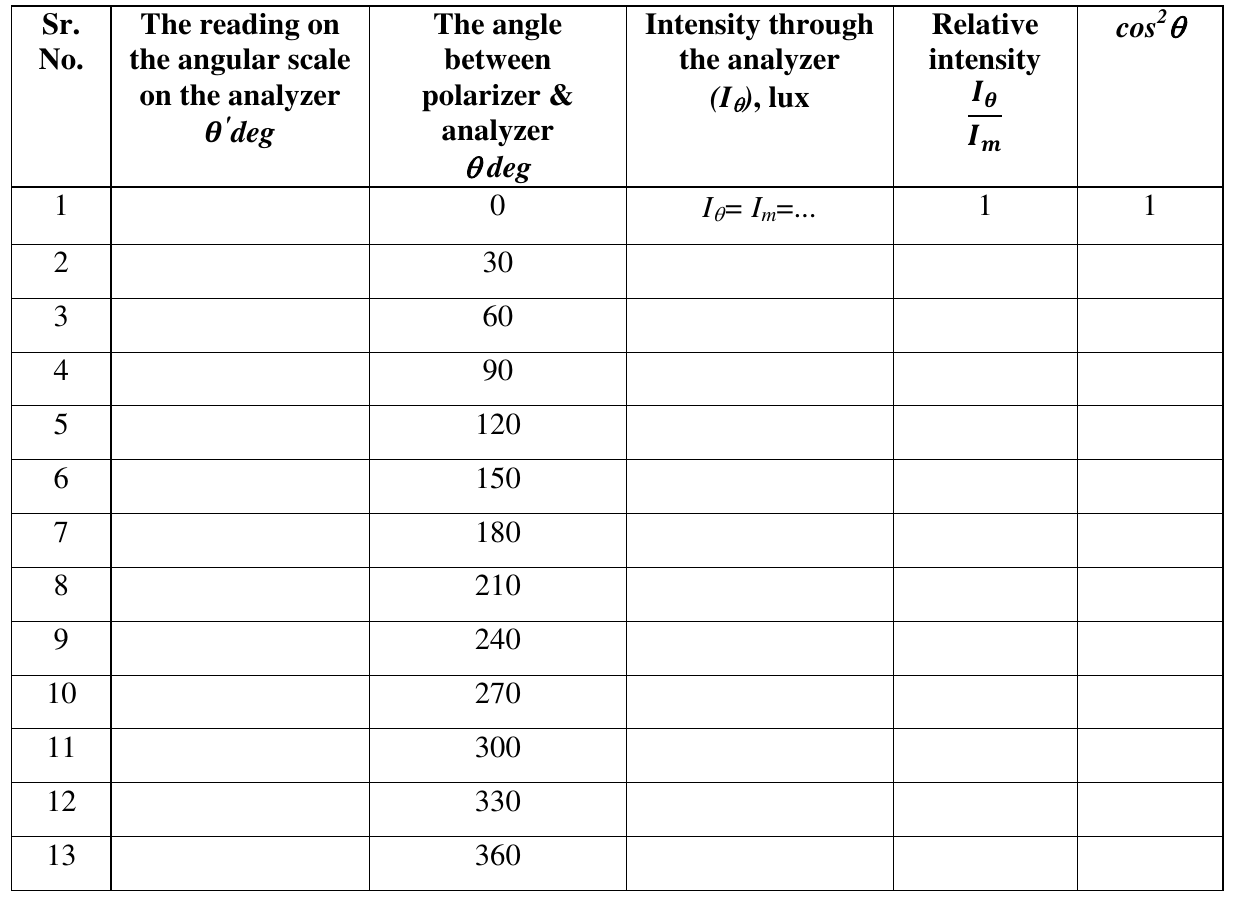
\includegraphics[scale=0.5]{table.png}
	\label{it}
\end{figure}

\section{Graphs}
\subsection{Plot between $I_\theta /I_m$ vs $\cos^2\theta$}
\begin{figure}[H]
	\centering
	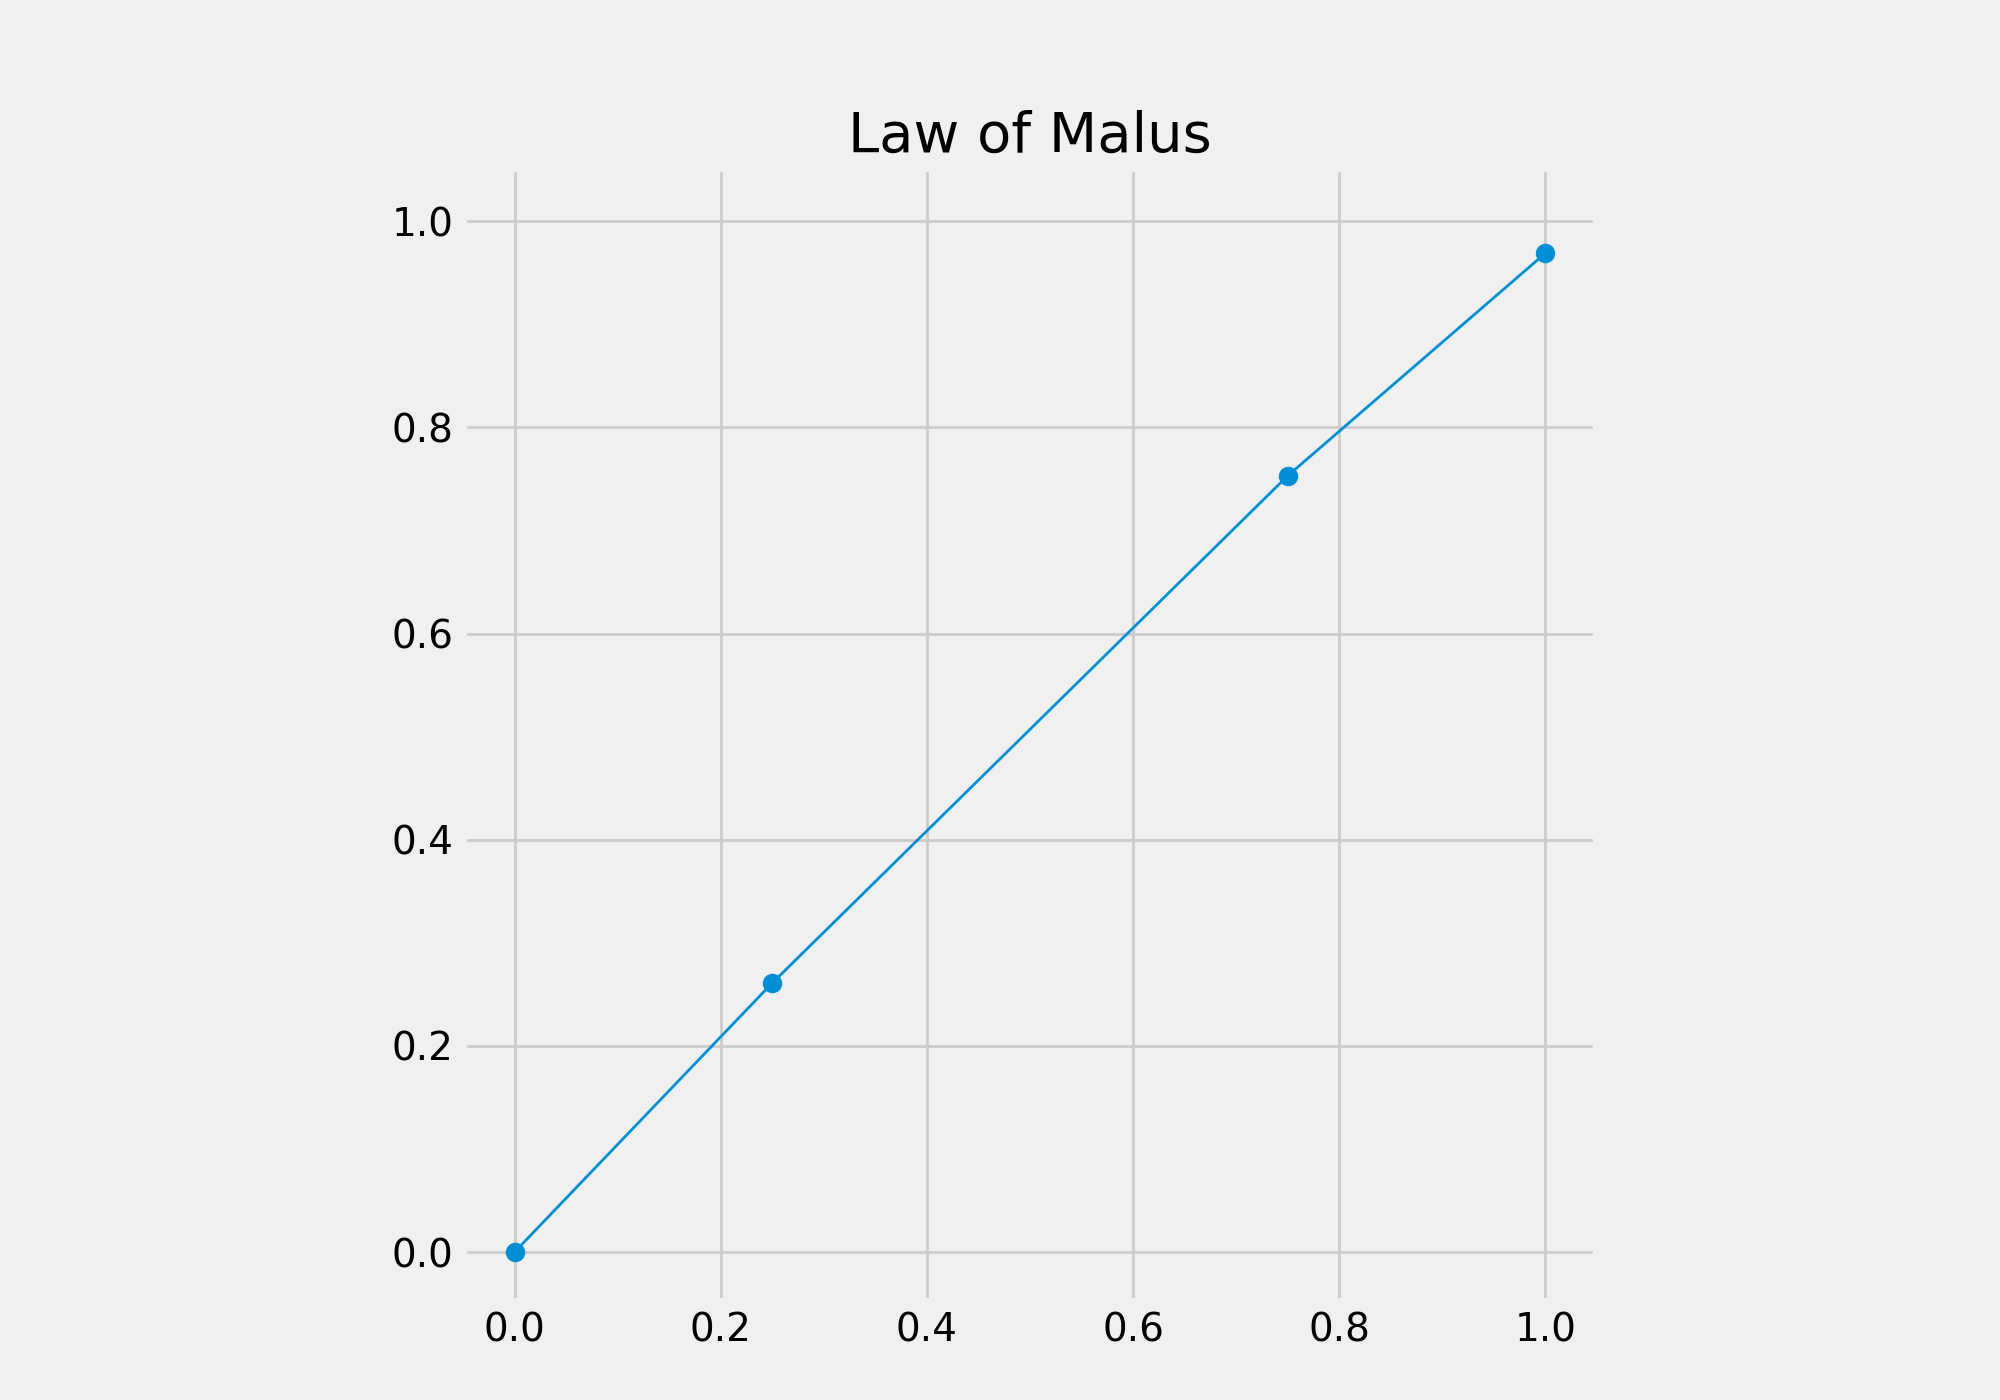
\includegraphics[scale=0.6]{plot2.png}
	\label{it}
\end{figure}

\subsection{Plot between $I_\theta /I_m$ vs $\theta$}
\begin{figure}[H]
	\centering
	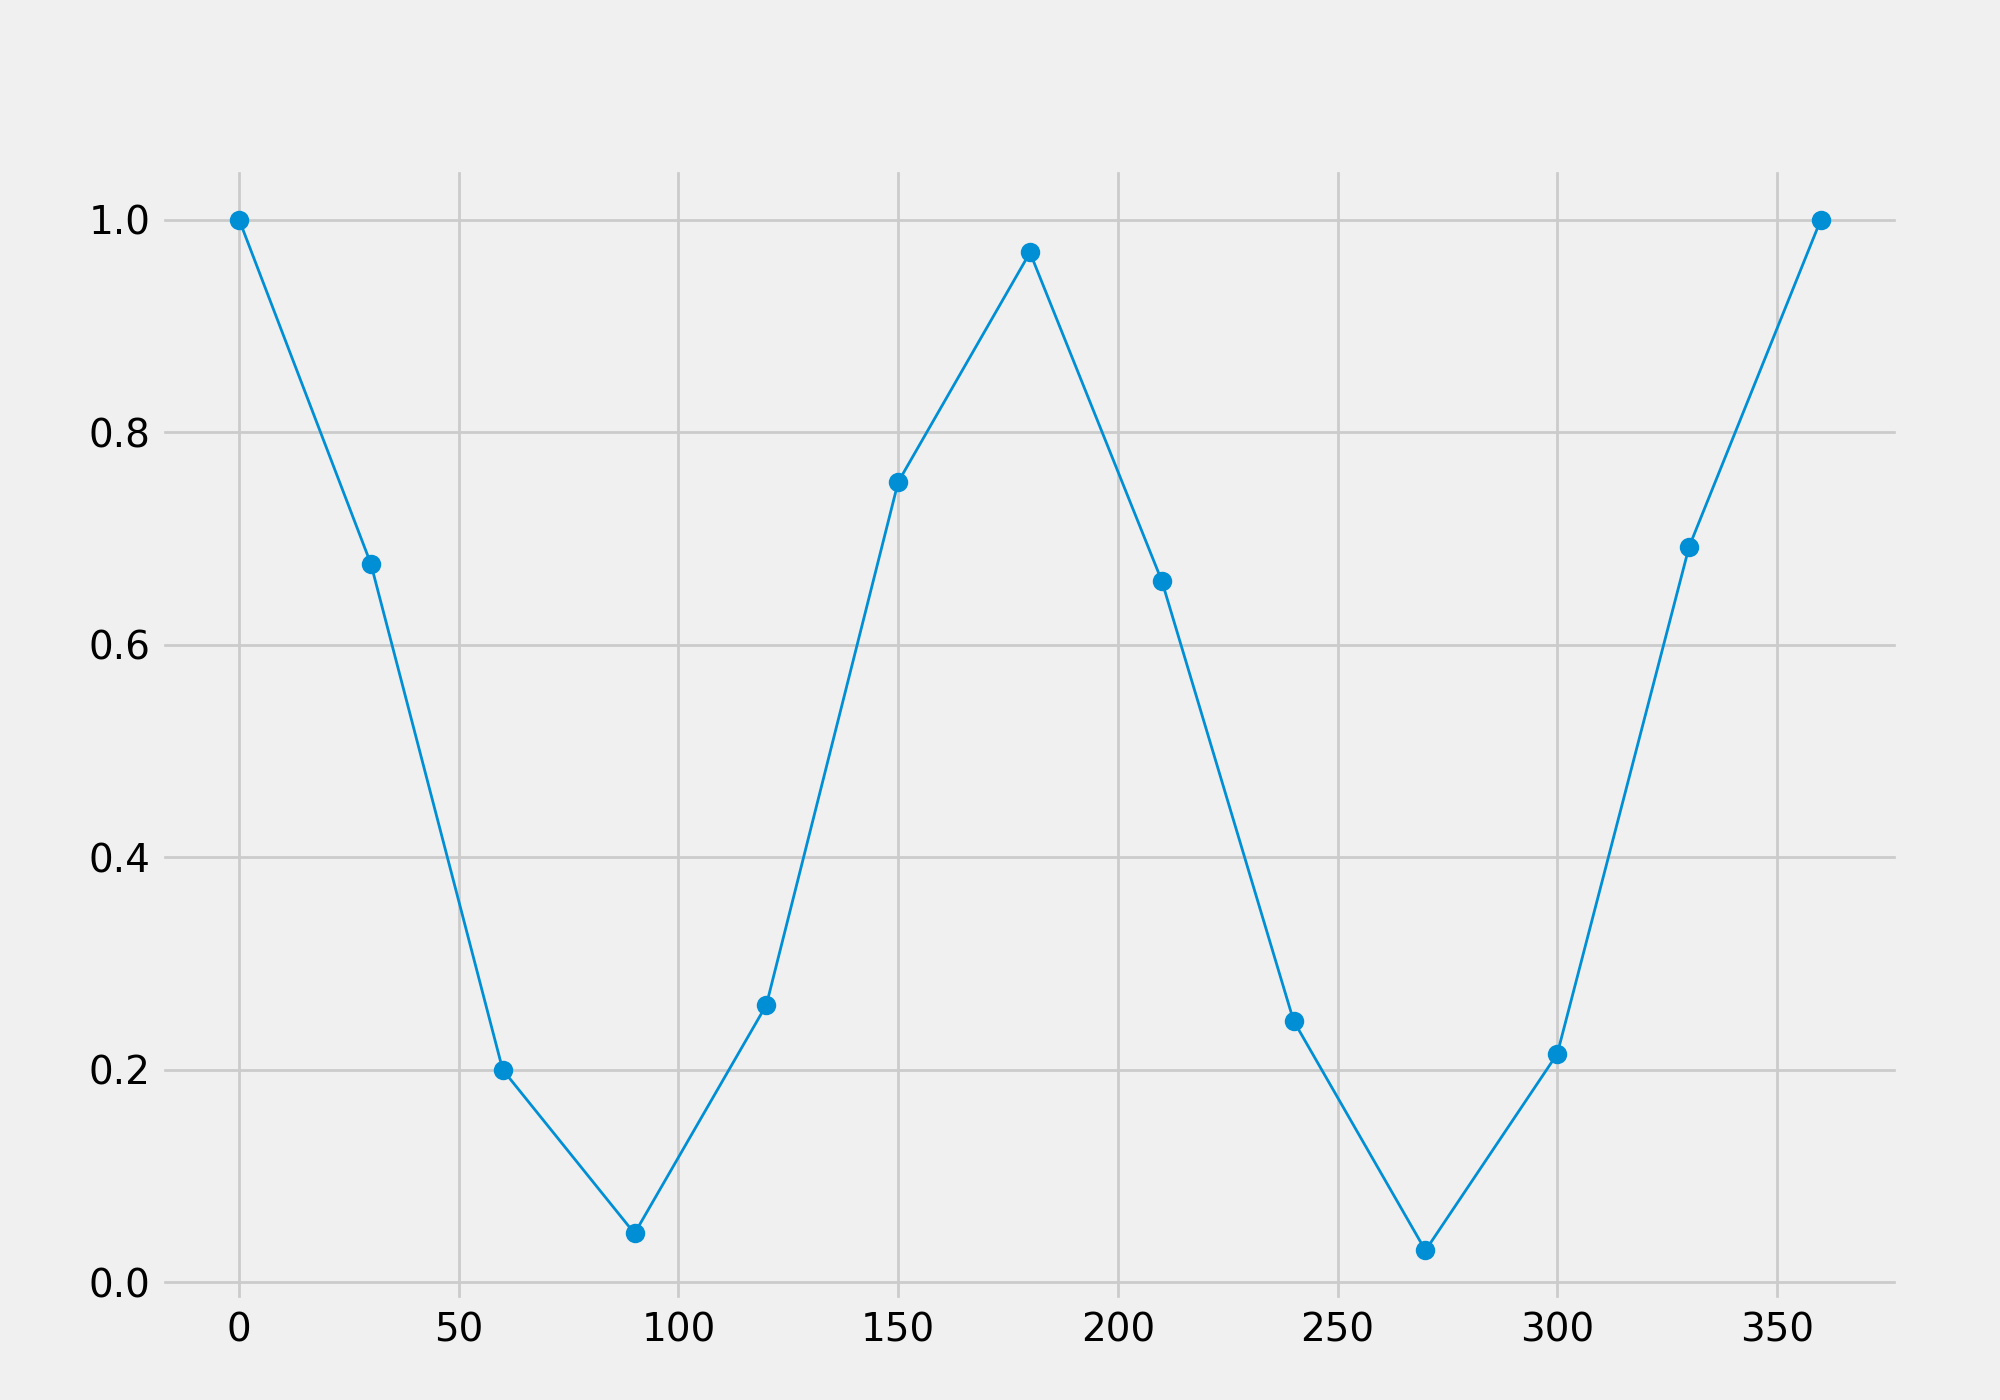
\includegraphics[scale=0.6]{plot_gg.png}
	\label{it}
\end{figure}

	\section{My Understanding of the Experiment}
	Law of Malus relates the intensity of light emitted from the analyzer to the polariser. This is important because it gives practical value to the role of the analyzer. By finding out the intensity of light obtained by the analyzer, one can conclude whether or not the light is polarized, partially polarised, or unpolarised. \textit{Therefore, that would be one of the main applications of this experiment. }
	
	If the light rays were polarized, then they would travel in the direction parallel to the optic axis of the polariser, and if the analyzer were kept on the same optic axis, or 180 $\deg$ to it, then the parallel components of light would pass through with the same intensity, and if not then it it would reduce by some factor, which is a function of the angle $\theta$ between the analyzer and the polarizer.

\end{document}